\PassOptionsToPackage{unicode=true}{hyperref} % options for packages loaded elsewhere
\PassOptionsToPackage{hyphens}{url}
%
\documentclass[]{book}
\usepackage{lmodern}
\usepackage{amssymb,amsmath}
\usepackage{ifxetex,ifluatex}
\usepackage{fixltx2e} % provides \textsubscript
\ifnum 0\ifxetex 1\fi\ifluatex 1\fi=0 % if pdftex
  \usepackage[T1]{fontenc}
  \usepackage[utf8]{inputenc}
  \usepackage{textcomp} % provides euro and other symbols
\else % if luatex or xelatex
  \usepackage{unicode-math}
  \defaultfontfeatures{Ligatures=TeX,Scale=MatchLowercase}
\fi
% use upquote if available, for straight quotes in verbatim environments
\IfFileExists{upquote.sty}{\usepackage{upquote}}{}
% use microtype if available
\IfFileExists{microtype.sty}{%
\usepackage[]{microtype}
\UseMicrotypeSet[protrusion]{basicmath} % disable protrusion for tt fonts
}{}
\IfFileExists{parskip.sty}{%
\usepackage{parskip}
}{% else
\setlength{\parindent}{0pt}
\setlength{\parskip}{6pt plus 2pt minus 1pt}
}
\usepackage{hyperref}
\hypersetup{
            pdftitle={Causality and Multiple Regression Supplement},
            pdfauthor={Krista Watts and Kevin Cummiskey},
            pdfborder={0 0 0},
            breaklinks=true}
\urlstyle{same}  % don't use monospace font for urls
\usepackage{color}
\usepackage{fancyvrb}
\newcommand{\VerbBar}{|}
\newcommand{\VERB}{\Verb[commandchars=\\\{\}]}
\DefineVerbatimEnvironment{Highlighting}{Verbatim}{commandchars=\\\{\}}
% Add ',fontsize=\small' for more characters per line
\usepackage{framed}
\definecolor{shadecolor}{RGB}{248,248,248}
\newenvironment{Shaded}{\begin{snugshade}}{\end{snugshade}}
\newcommand{\AlertTok}[1]{\textcolor[rgb]{0.94,0.16,0.16}{#1}}
\newcommand{\AnnotationTok}[1]{\textcolor[rgb]{0.56,0.35,0.01}{\textbf{\textit{#1}}}}
\newcommand{\AttributeTok}[1]{\textcolor[rgb]{0.77,0.63,0.00}{#1}}
\newcommand{\BaseNTok}[1]{\textcolor[rgb]{0.00,0.00,0.81}{#1}}
\newcommand{\BuiltInTok}[1]{#1}
\newcommand{\CharTok}[1]{\textcolor[rgb]{0.31,0.60,0.02}{#1}}
\newcommand{\CommentTok}[1]{\textcolor[rgb]{0.56,0.35,0.01}{\textit{#1}}}
\newcommand{\CommentVarTok}[1]{\textcolor[rgb]{0.56,0.35,0.01}{\textbf{\textit{#1}}}}
\newcommand{\ConstantTok}[1]{\textcolor[rgb]{0.00,0.00,0.00}{#1}}
\newcommand{\ControlFlowTok}[1]{\textcolor[rgb]{0.13,0.29,0.53}{\textbf{#1}}}
\newcommand{\DataTypeTok}[1]{\textcolor[rgb]{0.13,0.29,0.53}{#1}}
\newcommand{\DecValTok}[1]{\textcolor[rgb]{0.00,0.00,0.81}{#1}}
\newcommand{\DocumentationTok}[1]{\textcolor[rgb]{0.56,0.35,0.01}{\textbf{\textit{#1}}}}
\newcommand{\ErrorTok}[1]{\textcolor[rgb]{0.64,0.00,0.00}{\textbf{#1}}}
\newcommand{\ExtensionTok}[1]{#1}
\newcommand{\FloatTok}[1]{\textcolor[rgb]{0.00,0.00,0.81}{#1}}
\newcommand{\FunctionTok}[1]{\textcolor[rgb]{0.00,0.00,0.00}{#1}}
\newcommand{\ImportTok}[1]{#1}
\newcommand{\InformationTok}[1]{\textcolor[rgb]{0.56,0.35,0.01}{\textbf{\textit{#1}}}}
\newcommand{\KeywordTok}[1]{\textcolor[rgb]{0.13,0.29,0.53}{\textbf{#1}}}
\newcommand{\NormalTok}[1]{#1}
\newcommand{\OperatorTok}[1]{\textcolor[rgb]{0.81,0.36,0.00}{\textbf{#1}}}
\newcommand{\OtherTok}[1]{\textcolor[rgb]{0.56,0.35,0.01}{#1}}
\newcommand{\PreprocessorTok}[1]{\textcolor[rgb]{0.56,0.35,0.01}{\textit{#1}}}
\newcommand{\RegionMarkerTok}[1]{#1}
\newcommand{\SpecialCharTok}[1]{\textcolor[rgb]{0.00,0.00,0.00}{#1}}
\newcommand{\SpecialStringTok}[1]{\textcolor[rgb]{0.31,0.60,0.02}{#1}}
\newcommand{\StringTok}[1]{\textcolor[rgb]{0.31,0.60,0.02}{#1}}
\newcommand{\VariableTok}[1]{\textcolor[rgb]{0.00,0.00,0.00}{#1}}
\newcommand{\VerbatimStringTok}[1]{\textcolor[rgb]{0.31,0.60,0.02}{#1}}
\newcommand{\WarningTok}[1]{\textcolor[rgb]{0.56,0.35,0.01}{\textbf{\textit{#1}}}}
\usepackage{longtable,booktabs}
% Fix footnotes in tables (requires footnote package)
\IfFileExists{footnote.sty}{\usepackage{footnote}\makesavenoteenv{longtable}}{}
\usepackage{graphicx,grffile}
\makeatletter
\def\maxwidth{\ifdim\Gin@nat@width>\linewidth\linewidth\else\Gin@nat@width\fi}
\def\maxheight{\ifdim\Gin@nat@height>\textheight\textheight\else\Gin@nat@height\fi}
\makeatother
% Scale images if necessary, so that they will not overflow the page
% margins by default, and it is still possible to overwrite the defaults
% using explicit options in \includegraphics[width, height, ...]{}
\setkeys{Gin}{width=\maxwidth,height=\maxheight,keepaspectratio}
\setlength{\emergencystretch}{3em}  % prevent overfull lines
\providecommand{\tightlist}{%
  \setlength{\itemsep}{0pt}\setlength{\parskip}{0pt}}
\setcounter{secnumdepth}{5}
% Redefines (sub)paragraphs to behave more like sections
\ifx\paragraph\undefined\else
\let\oldparagraph\paragraph
\renewcommand{\paragraph}[1]{\oldparagraph{#1}\mbox{}}
\fi
\ifx\subparagraph\undefined\else
\let\oldsubparagraph\subparagraph
\renewcommand{\subparagraph}[1]{\oldsubparagraph{#1}\mbox{}}
\fi

% set default figure placement to htbp
\makeatletter
\def\fps@figure{htbp}
\makeatother

\usepackage{booktabs}
\usepackage[]{natbib}
\bibliographystyle{apalike}

\title{Causality and Multiple Regression Supplement}
\author{Krista Watts and Kevin Cummiskey}
\date{2021-05-21}

\begin{document}
\maketitle

{
\setcounter{tocdepth}{1}
\tableofcontents
}
\hypertarget{preface}{%
\chapter*{Preface}\label{preface}}
\addcontentsline{toc}{chapter}{Preface}

This etext is an introduction to causality in statistics and multivariable methods for students in their first college course in statistics. Traditionally, except for a terse warning from instructors that ``correlation does not imply causation'', students only encounter causality in statistics if they take graduate-level courses in certain disciplines (economics, epidemiology, etc.). However, given the ubiquity of data-driven arguments in modern society, a deeper understanding of drawing cause-and-effect conclusions from data is a core competency of college graduates and deserves attention in the liberal arts curriculum. For more on causality in the undergraduate curriculum, see our paper \citep{cummiskey2020causal} and others on this subject \citep{horton2015challenges, kaplan2018teaching, lubke2020we}.

After introducing concepts in causality, we use an example-based approach to multiple regression emphasizing how the scientific goal of the study impacts modeling decisions and interpretation of results. Prediction and cause-and-effect are the two main scientific goals of studies using multiple regression. These goals determine how researchers use and interpret models. However, this distinction is rarely made in introductory courses. Too often, multiple regression in the introductory course focuses on prediction and much of the ``thinking'' outsourced to algorithmic searches. This narrow focus on prediction deprives students of the opportunity to exercise critical judgment and creativity. On the other hand, cause-and-effect studies require tying subject matter knowledge to developing causal models. During this process, students have to carefully consider relationships between variables (which is not particularly important in prediction), thus developing multivariable thinking, an important goal of the revised GAISE report \citep{carver2016guidelines}. Our approach to multiple regression uses the scientific goal to motivate how we think about our data and models. \citet{hernan2019second} argue for this approach in data science education; we believe it is appropriate for introductory statistics courses also.

This etext is appropriate for a wide variety of introductory statistics courses including both algrebra-based and calculus-based courses. It assumes students understand basic concepts in data analysis, inference (confidence intervals and statistical tests for means and proportions), and simple linear regression.

\hypertarget{introduction}{%
\chapter{Introduction}\label{introduction}}

\hypertarget{goals-of-quantitative-research-describe-predict-cause-and-effect}{%
\section{Goals of quantitative research (describe, predict, cause-and-effect)}\label{goals-of-quantitative-research-describe-predict-cause-and-effect}}

Researchers and practitioners employ quantitative methods to answer important questions and make decisions. Regardless of the discipline or application, they typically have one of three goals \citep{cozby2020methods}:

\begin{itemize}
\item
  \textbf{describe}
\item
  \textbf{predict}
\item
  \textbf{cause-and-effect}
\end{itemize}

Consider medical researchers investigating a newly discovered variant of the coronavirus. Initially, they might focus on describe studies. \emph{How prevalent is the variant in the population? How does the prevalence vary over space and time? What groups of individuals are most vulnerable to the variant? What else is associated with the variant?} Together, these studies help researchers better understand the variant and identify important variables for refined predict studies.

Predict studies identify individuals most at risk for the variant or for transmitting it to others. Researchers select potential predictors as inputs to algorithms and statistical methods that transform them into estimates of each individual's risk for the variant. These methods rely upon associations between the inputs and the variant. In addition, these methods estimate the error associated with their predictions. Researchers try to ensure error estimates obtained within their study are good estimates of the error when their models are applied to other populations. While predict studies help us identify who is at risk, they do not tell us the effect if we change something about individuals (quit smoking, lose weight, etc.) To answer these ``what if?'' questions, researchers use cause-and-effect studies.

Cause-and-effect studies try to estimate the effect of intervening or changing some aspect of an individual. These studies are tremendously important in public policy (where they are aptly called \emph{intervention studies}) to justify legislation and regulations to reduce risk. Unlike prediction studies, which are highly algorithmic and only require researchers to identify appropriate inputs, cause-and-effect studies use subject matter knowledge of the causal structure of the inputs to select appropriate statistical models \citep{hernan2019second}. For example, to assess the affect of quitting smoking on risk for the variant, we need to understand why some people quit smoking and others do not, as these reasons themselves may be responsible for some changes in risk between the two groups. Unlike prediction studies which rely upon what we \emph{see}, cause-and-effect studies require us to ask what would happen if we \emph{do} something \citep{pearl2018book}. Only human beings are capable of such counterfactual thinking (``what would have happened if'') - even our most sophisticated computer algorithms require human supervision to address cause-and-effect questions.

\hypertarget{validity}{%
\section{Validity}\label{validity}}

When designing a study, researchers carefully consider its internal and external validity.

\begin{itemize}
\item
  internal validity - How well does the study establish a cause-and-effect relationship between a treatment and outcome?
\item
  external validity - How broadly can the study's results be applied?
\end{itemize}

Often, there is a trade off between internal and external validity when designing a study. For example, to increase internal validity, researchers sometimes restrict the study to a subset of similar subjects to eliminate the effects of other variables. However, in doing so, they reduce the external validity of the study if the results do not apply to the other subjects. In an area of research, our knowledge comes from many studies with different levels of internal and external validity -- rarely does a single study answer every question. Consider the recent development of Covid-19 vaccines. For example, initial Covid-19 vaccine trials focused on internal validity to understand its effectiveness against the virus and obtain approval for mass distribution. \citet{polack2020safety} randomly assigned 43,548 persons 16 years of age or older to receive two doses of either placebo or the BNT162b2 vaccine (Pfizer). They observed eight cases of Covid-19 among participants who received BNT162b2 and 162 cases among those who received the placebo. This was a huge moment in the pandemic! Randomly assigning subjects to receive the vaccine increased the internal validity of the study. However, for ethical reasons, the subjects had to be relatively healthy and volunteer for the trials. These limitations reduced the external validity of the study because it is not clear whether the vaccine has the same effect in the general population. However, conducting more randomized trials on other populations has ethical implications of its own, as they would require withholding the vaccine from large segments of the population. In this case, an observational study is more appropriate.

\citet{dagan2021bnt162b2} conducted an observational study after the mass vaccination campaign in Israel using the health records of 4.7 million patients enrolled in its largest integrated health care organization. The researchers matched vaccine recipients to controls on important variables: age, sex, sector, neighborhood of residence, etc.. In this larger sample, they found vaccine effectiveness results consistent with the randomized trial, thus providing evidence of the vaccine's effectiveness in the general public. The authors specifically address the importance of observational studies:

\begin{quote}
``Although randomized clinical trials {[}experiments{]} are considered the ``gold standard'' for evaluating intervention effects, they have notable limitations of sample size and subgroup analysis, restrictive inclusion criteria, and a highly controlled setting that may not be replicated in a mass vaccine rollout."
\end{quote}

\textbf{Exercises}

\begin{enumerate}
\def\labelenumi{\arabic{enumi}.}
\tightlist
\item
  For the following studies, identify the goal (describe, predict, cause-and-effect) of the study. Briefly explain your choice:
\end{enumerate}

\begin{itemize}
\item
  \emph{A researcher obtains school records to collect information on the extracurricular activities of students.}
\item
  \emph{A researcher obtains school records to determine the impact of extracurricular activities on grades.}
\item
  \emph{A researcher obtains school records on extracurricular activities to identify students who are at risk to graduate.}
\end{itemize}

\begin{enumerate}
\def\labelenumi{\arabic{enumi}.}
\setcounter{enumi}{1}
\item
  Select an area of interest to you. Write a sentence describing a study in your area of interest for each of the three goals (describe, predict, cause-and-effect).
\item
  Read the article \href{https://www.nature.com/articles/d41586-020-02821-4}{``Dozens to be deliberately infected with coronavirus in UK `human challenge' trials''} in Nature News. Write a paragraph discussing issues of internal and external validity.
\end{enumerate}

\hypertarget{causality}{%
\chapter{Causality}\label{causality}}

There was a revolution over the last three decades in how scientists view causality. A hundred years ago, when the statistical methods we learn in introductory courses were developed, causality was considered outside the realm of statistics, except for the case of randomized controlled experiments. In other words, statistics could only answer questions of association, but not of causality. However, this limited view of statistics was at odds with its usage in every day research. For example, the greatest public health triumph of the 20th century was the reduction in cigarette smoking, which exploded after World War II with their mass production and marketing. The statistical evidence of the health effects of smoking comes entirely from observational studies -- there has never been a randomized controlled trial for smoking. The \href{https://www.cancer.org/latest-news/the-study-that-helped-spur-the-us-stop-smoking-movement.html}{American Cancer Society's observational studies} beginning in the 1950's were huge undertakings and provided compelling evidence of the harmful effects of cigarette smoking \citep{hammond1954relationship, hammond1966smoking}. Clearly, statistical theory and practice had diverged in their understandings of causality.

However, in the 1980's and 1990's, researchers in different disciplines began revisiting causality \citep{greenland1986identifiability, pearl1993bayesian, angrist1995identification}. They developed mathematical language for expressing causation, which cannot be uniquely expressed using the traditional language of association. In addition, they showed randomized controlled trials are special cases of more general situations when the researcher has full knowledge of the assignment mechanism. The \emph{assignment mechanism} is the process in which subjects are assigned to different levels of the treatment. Lastly, they showed that causal effects can be estimated from observational studies under a wide variety of circumstances when the assignment mechanism is known. Today, while ``correlation does not imply causation'' is still useful advice when assessing causal claims in observational studies, statistical theory and practice suggest our assessment of causal claims should be richer and more nuanced than this simple rule of thumb.

\hypertarget{what-does-it-mean-for-one-thing-to-cause-another}{%
\section{What does it mean for one thing to cause another}\label{what-does-it-mean-for-one-thing-to-cause-another}}

We say one variable (called the treatment, exposure, or intervention) \emph{causes} another variable (the outcome or response) if there is a change in the average outcome between subjects when they receive the treatment and the same subjects when they do not receive the treatment. This definition differs from \emph{association}, which is a change in the average outcome between subjects who received the treatment and different subjects who did not receive the treatment. Thus, causation is a comparison of observed outcomes and their counterfactuals (``what would have happened if the subject were in the other treatment group'').

The central challenge in assessing causality is that we cannot observe the outcomes for subjects under both levels of the treatment variable. In other words, we only get to observe each subject in either the treatment or the control group. For example, when estimating the effect of smoking on long term health outcomes, it is impossible to observe the same subject as a smoker and as a nonsmoker. However, under certain circumstances, we can obtain good estimates of effects without observing both outcomes for each individual. The most famous of these is the randomized controlled experiment.

\hypertarget{randomized-controlled-experiments}{%
\section{Randomized controlled experiments}\label{randomized-controlled-experiments}}

One of the most important scientific discoveries of the early 20th century was the randomized controlled trial (RCT). In its simplest form, researchers randomly assign subjects to receive the treatment or be in the control group. If they observe a difference in average outcomes between the two groups, then we would say the treatment caused the outcome. \emph{Why does assigning subjects to groups by the simple action of flipping a coin result in such a radical difference in how we interpret the results?} The answer lies in the definition of causation above. Causation compares the outcomes between the same subjects. When we randomize the treatment, we compare the outcome in one group of subjects with the treatment to another group of subjects without the treatment who we expect to be very similar. In fact, when we have large enough sample sizes, it would be very unusual for the two groups to differ much. We refer to the two groups as \emph{exchangeble}. In other words, we would expect the control group to have had similar results as the treatment group if they were the treatment group, and vice versa.

However, an overly restrictive view of causality followed this important discovery. That is, causality can \emph{only} be shown with RCTs. This placed a huge limitation on the types of research questions statistics could address. Frequently, RCTs are not ethical, feasible, or desirable. Would you enroll in a study where you could be randomly assigned to be a smoker for the next 20 years? Towards the end of the 20th century, researchers began taking a more expansive view of causality in observational studies.

\hypertarget{observational-studies-and-confounding}{%
\section{Observational Studies and Confounding}\label{observational-studies-and-confounding}}

In observational studies, researchers do not intervene on the assignment of subjects to treatment and control groups. (Note: a common misconception is that observational studies do not have treatment and control groups. This is not true. The distinction between randomized controlled experiments and observational studies is about how subjects are \emph{assigned} to the treatment groups.) Instead, other factors determine subjects' treatment group assignment. For example, adolescents with a history of abuse, family violence, and stressful life events are more likely to smoke \citep{ellickson2001high, simantov2000health}.

\emph{Confounding} occurs when these other factors determining assignment are themselves causes of the outcome. In other words, the treatment and control groups are different in ways that are important to the outcome. The two groups are not exchangeable. An observed association between the treatment and outcome could mean (1) the treatment caused the outcome, (2) other factors causing group assignment caused the outcome, or (3) both. Furthermore, with only information on the treatment and outcome, it is not possible to identify which of the three is the correct explanation. Confounding is a form of statistical bias -- using the observed association as an estimate of the treatment effect will be systemically off. Increasing the sample size does not fix bias, you just get a more precise, wrong estimate.

For example, consider an observational study investigating long term health effects of smoking. In many populations, males are more likely to be smokers. In addition, males have different risks for long term health outcomes than females, regardless of whether they smoke. If we observe an association between smoking and an outcome without information on sex, we cannot distinguish the effect of smoking from the effect of sex.

However, researchers in the late 20th century had a key insight. If we know the assignment mechanism and measure a sufficient set of confounding variables, we can obtain good estimates of treatment effects from observational studies. This was huge! Observational studies and RCTs are not fundamentally different. Estimating effects requires understanding the assignment mechanism, and RCTs are just a special case with a simple, known assignment mechanism. Given this insight, researchers became more comfortable making causal claims from observational studies when they have knowledge of the assignment mechanism. \emph{How do we identify a sufficient set of confounding variables?} For that question, we turn to causal diagrams.

\hypertarget{causal-diagrams}{%
\section{Causal Diagrams}\label{causal-diagrams}}

Causal diagrams are useful tools for depicting the assignment mechanism (also called the causal model). Experts use subject matter knowledge in their field to specify the causal model. They typically specify the causal model prior to collecting data to identify confounding variables to measure. Importantly, there is no way to determine the presence of unmeasured confounding using the data. Using simple heuristics for causal diagrams, they help identify a sufficient set of confounding variables to control for during design and analysis.

Causal diagrams are directed, acyclic graphs (DAGs) where the nodes are variables. A directed edge (arrow) connecting two nodes indicates the node at the arrow's tail is a cause of the node at the arrow's head. The graphs are directed because the arrows point in one direction. They are acyclic because you can never get back to where you started by following arrows. The convention in many disciplines is to order the variables temporally from left to right -- we adopt that convention here.

There are three types of variables that are the building blocks of causal diagrams.

\hypertarget{confounding-variable}{%
\subsection{Confounding variable}\label{confounding-variable}}

Figure \ref{fig:confounder} depicts the confounding variable \(C\) of the effect of treatment \(X\) on outcome \(Y\). We say there is a \emph{backdoor path} between \(X\) and \(Y\) through \(C\). We will observe an association between \(X\) and \(Y\) even if there is no treatment effect. The levels of \(X\) differ in terms of \(C\) and \(C\) itself is a cause of \(Y\). Without measuring and controlling for \(C\), we cannot distinguish the effect of \(X\) on \(Y\) from the association through confounding variable \(C\). However, if \(C\) is the only confounding variable, controlling for it will result in good estimates of the effect of \(X\) on \(Y\). When we control for \(C\), we say the backdoor path from \(X\) to \(Y\) is ``blocked''.

\begin{figure}
\centering
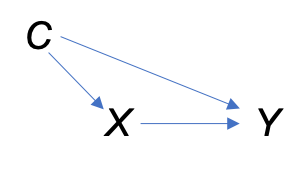
\includegraphics{./images/confounder.png}
\caption{\label{fig:confounder} A confounding variable \(C\) on the effect of \(X\) on \(Y\).}
\end{figure}

For example, let's say researchers investigate the effect of a master's degree on adult earnings. They survey a large number of individuals and record whether they have a master's degree and their earnings. Socioeconomic status is a confounding variable. Individuals with higher socioeconomic status are more likely to earn master's degrees. In addition, they are more likely to have higher adult earnings, regardless of whether they have a master's degree. For this example, let's assume socioeconomic status is the only confounding variable. If the researchers observe an association between master's degrees and earnings without information on socioeconomic status, it is not possible to determine if the association is due to an effect of master's degrees or the effect of socioeconomic status.

\hypertarget{collider}{%
\subsection{Collider}\label{collider}}

Figure \ref{fig:collider} depicts treatment \(X\) with no effect on outcome \(Y\). \(X\) and \(Y\) are both causes of collider \(Z\) (the two incoming arrows \emph{collide}). The box around \(Z\) indicates conditioning upon \(Z\) in the analysis. In this case, there will be an association between \(X\) and \(Y\) even though there is no treatment effect. Figure \ref{fig:collider} is a common way to depict \emph{selection bias} where an association in subjects selected for the study is not present in the general population. In the selection bias diagram, \(Z\) is an indicator of selection into the study with a box around it because researchers only observe subjects selected into the study.

\begin{figure}
\centering
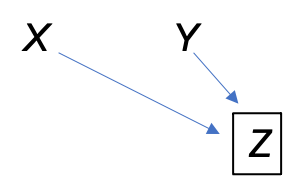
\includegraphics{./images/collider.png}
\caption{\label{fig:collider} Collider \(Z\) with no treatment effect of \(X\) on \(Y\).}
\end{figure}

A very famous example appears in \citet{pearl2018book}. In the general population, we would not expect to see an association between an individual's talent and looks. More talented people are not better looking and vice versa. However, if we look only at famous Hollywood actors (\(Z\)), we would see a negative association between talent and looks in this group because an individual needs either talent or looks (or both) to become a famous Hollywood actor. Being less talented makes it more likely the actor is good looking because there must be some reason they became a famous Hollywood actor. More seriously, \emph{selection bias} is a huge issue in medical and public health studies resulting in easily misinterpretated associations \citep{hernan2004structural, cole2010illustrating, elwert2014endogenous}. For example, several studies have found a protective effect of smoking on Covid-19 infections (see Exercises).

\hypertarget{mediator}{%
\subsection{Mediator}\label{mediator}}

Figure \ref{fig:mediator} depicts mediator \(M\) of the effect of treatment \(X\) on outcome \(Y\). In this case, \(X\) is a cause of \(M\), \(M\) is a cause of \(Y\), and there is no effect of \(X\) on \(Y\) that cannot be explained by the effect of \(M\) on \(Y\). A common mistake is to adjust for \(M\). If we adjust for \(M\), we will not observe an association between \(X\) and \(Y\) when there is an effect of \(X\) on \(Y\).

\begin{figure}
\centering
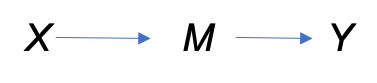
\includegraphics{./images/mediator.png}
\caption{\label{fig:mediator} Mediator \(M\) of the effect of treament \(X\) on outcome \(Y\).}
\end{figure}

For example, let's say researchers are investigating an adverse reaction to a medication using a treatment group and a control group where the adverse reactions are always preceded by increased blood pressure. Even if there is an effect of the medication on the adverse reaction, when we condition upon experiencing increased blood pressure, we will not observe an association between the medication and adverse reactions. Unfortunately, some researchers condition upon everything they measure, often resulting in poor estimates of effects \citep{hernan2002causal}.

\textbf{Exercises}

\begin{enumerate}
\def\labelenumi{\arabic{enumi}.}
\tightlist
\item
  You investigate the effect of a college education on adult earnings by surveying 1000 adults in your area and ask them if they have a bachelor's degree (Y/N) and their yearly income in dollars. You find the college graduates earn about \$30,000 more per year on average than the high school graduates.
\end{enumerate}

\begin{enumerate}
\def\labelenumi{\alph{enumi})}
\item
  Name the treatment and outcome variables in your study.
\item
  Is this an observational study or randomized controlled experiment? Explain.
\item
  Explain what it means for college education to cause higher adult earnings. In addition, explain how this differs from college education being associated with higher adult earnings.
\item
  Identify and explain a potential confounding variable in your study. (Be sure to explain how your confonding variable is a common cause of both the treatment and outcome).
\item
  Draw a causal diagram depicting the relationship between the treatment, outcome, and your confounding variable.
\item
  You also ask whether the individual has a Master's degree (Y/N). What type of variable is having a Master's degree? Redraw your diagram with this variable included in it.
\end{enumerate}

\begin{enumerate}
\def\labelenumi{\arabic{enumi}.}
\setcounter{enumi}{1}
\tightlist
\item
  Several studies have found a negative association between smoking and Covid-19 infection. Read \href{https://rss.onlinelibrary.wiley.com/doi/10.1111/1740-9713.01413}{``The spectre of Berkson's paradox: Collider bias in Covid-19 research''} and answer the following questions.
\end{enumerate}

\begin{enumerate}
\def\labelenumi{\alph{enumi})}
\item
  Explain what it means for smoking to cause a reduction in Covid-19 infections.
\item
  What type of variable is hospitalization in Figure 2?
\item
  Explain why many studies observe a negative association between smoking and Covid-19 infection.
\end{enumerate}

\hypertarget{confounding-adjustment-with-regression}{%
\chapter{Confounding adjustment with regression}\label{confounding-adjustment-with-regression}}

Recall from Chapter 2 that confounding occurs when the treatment variable depends upon another variable that is itself a cause of the outcome. When researchers have not controlled for a confounding variable through study design, they employ statistical methods during analysis to adjust for confounding. One of the most common techniques is multiple regression.

\hypertarget{categorical-confounding-variable}{%
\section{Categorical confounding variable}\label{categorical-confounding-variable}}

Let's say we have treatment variable (X) and response variable (Y) but the relationship between them is confounded by a third variable (C). For instance, suppose we want to investigate the relationship between ice cream sales and hospital admissions for heart attacks in the summer in NYC. In this example, our ``treatment'' is volume of ice cream sales on any given day in NYC and our response is number of hospital admissions that day for heart attacks. If we only look at those two variables, we might see a strong correlation; as ice cream sales increase, so do heart attacks. But it would be a mistake to infer that eating ice cream causes heart attacks from this analysis alone.

What does it mean for ice cream sales to \emph{cause} heart attacks? How is that different from an association between ice cream sales and heart attacks? Ice cream sales cause heart attacks if high and low ice cream sales on the same days resulted in different heart attack rates. However, we only get to observe each day with one value of ice cream sales. Therefore, a third variable may be a common cause of both ice cream sales and heart attacks. In this case, we say there is an association between ice cream sales and heart attacks.

In our case, the third variable is temperature. People tend to buy more ice cream when it is hot; if there also tends to be more heart attacks when it is hot, temperature confounds the relationship between ice cream sales and hospital admissions for heart attack. Recall the confounding diagram from Chapter 2. If we extend it to this example, we have

\begin{figure}
\centering
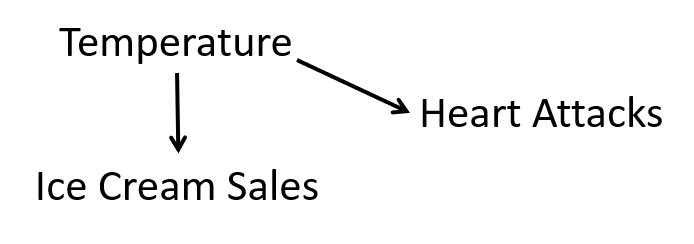
\includegraphics{./images/ice_cream_graph.png}
\caption{Causal diagram for ice cream sales and heart attacks.}
\end{figure}

Notice that we believe that a change in temperature \emph{causes} a change in both ice cream sales and heart attacks.

If we control for temperature, then we will no longer see an association between ice cream sales and heart attacks. One way to control for temperature is to restrict the analysis to only days in a very narrow temperature range. However, restricting your analysis in this way would result in a lot of lost information. Instead, we turn to statistical methods like regression.

\hypertarget{unadjusted-effect-of-x-on-y}{%
\subsection{\texorpdfstring{Unadjusted effect of \(X\) on \(Y\)}{Unadjusted effect of X on Y}}\label{unadjusted-effect-of-x-on-y}}

There exists a belief that height is protective against high blood pressure; that is, taller people tend to have lower blood pressure. In this section, we investigate this belief using data gathered from 1999 to 2006 by the CDC's National Health and Nutrition Examination Survey (NHANES), a (relatively) representative sample of the adult U.S. population. The data contains variables on 12,671 Americans age 18 and older who were not pregnant or taking high blood pressure medication. We are interested in estimating the effect of height (HT) on mean systolic blood pressure (SBP). We could model this with the following regression equation.
\[\widehat{SBP}=\beta_0+\beta_1*HT\]

If we fit a regression model with height as the treatment variable and systolic blood pressure as the response, we get the following results:

\begin{Shaded}
\begin{Highlighting}[]
\NormalTok{bp_dat<-}\KeywordTok{read_csv}\NormalTok{(}\StringTok{"./data/blood_pressure.csv"}\NormalTok{)}
\NormalTok{ht_mod=}\KeywordTok{lm}\NormalTok{(SBP}\OperatorTok{~}\NormalTok{HT,}
         \DataTypeTok{data =}\NormalTok{ bp_dat)}
\KeywordTok{summary}\NormalTok{(ht_mod)}
\end{Highlighting}
\end{Shaded}

\begin{verbatim}
## 
## Call:
## lm(formula = SBP ~ HT, data = bp_dat)
## 
## Residuals:
##     Min      1Q  Median      3Q     Max 
## -52.876 -13.804  -3.703   9.922 141.605 
## 
## Coefficients:
##              Estimate Std. Error t value Pr(>|t|)    
## (Intercept) 141.22705    2.52887  55.846  < 2e-16 ***
## HT           -0.10276    0.01504  -6.833 8.58e-12 ***
## ---
## Signif. codes:  0 '***' 0.001 '**' 0.01 '*' 0.05 '.' 0.1 ' ' 1
## 
## Residual standard error: 20.09 on 17486 degrees of freedom
## Multiple R-squared:  0.002663,   Adjusted R-squared:  0.002606 
## F-statistic: 46.69 on 1 and 17486 DF,  p-value: 8.575e-12
\end{verbatim}

Note the coefficient on height is actually positive, meaning that taller people actually tend to have higher blood pressure! In fact, we expect SBP to go up by about 0.05 mmHG for every cm in additional height. This makes sense when we look at the data. There is A LOT of data here, but we see a general increase in SBP as height increases.

\begin{Shaded}
\begin{Highlighting}[]
\NormalTok{bp_dat}\OperatorTok
\StringTok{  }\KeywordTok{ggplot}\NormalTok{(}\KeywordTok{aes}\NormalTok{(}\DataTypeTok{x=}\StringTok{`}\DataTypeTok{HT}\StringTok{`}\NormalTok{,}
             \DataTypeTok{y=}\StringTok{`}\DataTypeTok{SBP}\StringTok{`}\NormalTok{))}\OperatorTok{+}
\StringTok{  }\KeywordTok{geom_point}\NormalTok{()}\OperatorTok{+}
\StringTok{  }\KeywordTok{theme_classic}\NormalTok{()}
\end{Highlighting}
\end{Shaded}

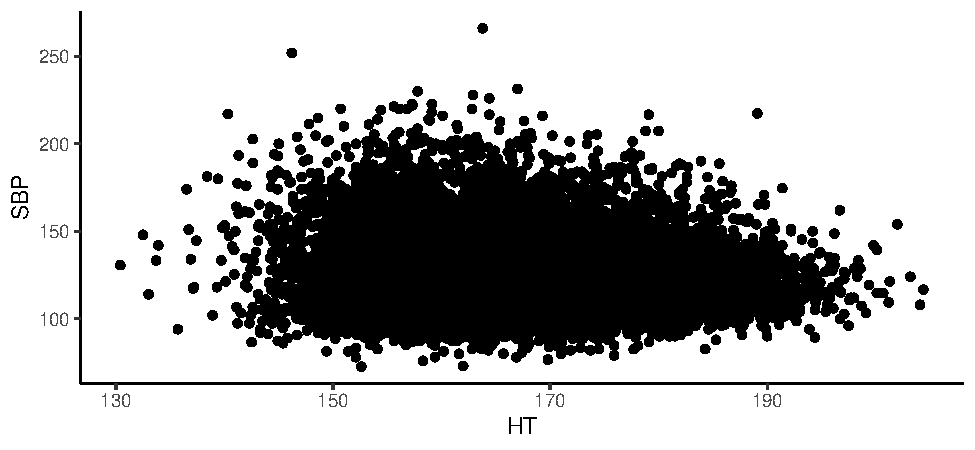
\includegraphics{MA206supplement_files/figure-latex/unnamed-chunk-4-1.pdf}

This is contrary to what we expected. So I guess previous research was wrong. Wait -- not so fast. Biological sex is a potential confounder.

\hypertarget{effect-of-x-on-y-adjusting-for-c}{%
\subsection{\texorpdfstring{Effect of \(X\) on \(Y\) adjusting for \(C\)}{Effect of X on Y adjusting for C}}\label{effect-of-x-on-y-adjusting-for-c}}

Men tend to be taller than women (175 cm vs 162cm). Men also tend to have higher mean systolic blood pressure (122 vs 118 mmHG). Therefore, Sex is a possible confounder. Below is our data, colored by Sex.

\begin{Shaded}
\begin{Highlighting}[]
\NormalTok{bp_dat}\OperatorTok
\StringTok{  }\KeywordTok{ggplot}\NormalTok{(}\KeywordTok{aes}\NormalTok{(}\DataTypeTok{x=}\StringTok{`}\DataTypeTok{HT}\StringTok{`}\NormalTok{,}
             \DataTypeTok{y=}\StringTok{`}\DataTypeTok{SBP}\StringTok{`}\NormalTok{))}\OperatorTok{+}
\StringTok{  }\KeywordTok{geom_point}\NormalTok{(}\KeywordTok{aes}\NormalTok{(}\DataTypeTok{colour =}\NormalTok{ SEX))}\OperatorTok{+}
\StringTok{  }\KeywordTok{theme_classic}\NormalTok{()}
\end{Highlighting}
\end{Shaded}

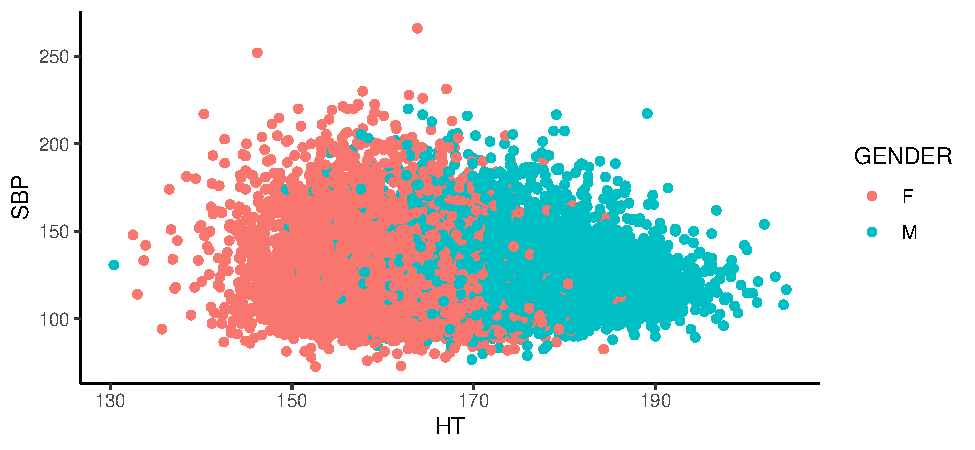
\includegraphics{MA206supplement_files/figure-latex/unnamed-chunk-5-1.pdf}

Here, we see SBP tends to decrease as height increases \emph{within men}. Likewise, \emph{within women}, we see the same. If we want to estimate the effect of height on blood pressure, we must first adjust for Sex. We do this using multiple regression. ``Multiple'' because we have multiple variables on the right hand side of the equation. (This could be multiple explanatory variables or, as we have here a single explanatory variable with one or more confounding variables.) Often we do this simply by adding the other variable to the regression equation. But how do we add a categorical variable to a mathematical equation. Suppose my regression model is

\[\widehat{SBP}=\beta_0+\beta_1*HT+\beta_2*SEX\]

What does it mean to multiply something by ``male''? When we want to include categorical variables as explanatory variables in regression models, we often use indicator (also called `dummy') variables. In this case, biological sex has two levels, male and female, and we need one indicator variable to represent Sex. We will let our indicator variable equal 1 if a subject was male and 0 if the subject was female. \(\beta_2\) is interpreted as the expected increase in SBP when a subject is male.

A possible multiple regression equation with SBP as our response, height as the treatment adjusting for Sex as a confounder is

\[\widehat{SBP}=\beta_0+\beta_1*HT+\beta_2*SEX\]

When we add Sex to the model, we get the following results.

\begin{Shaded}
\begin{Highlighting}[]
\NormalTok{ht_gen_mod=}\KeywordTok{lm}\NormalTok{(SBP}\OperatorTok{~}\NormalTok{HT}\OperatorTok{+}\NormalTok{SEX,}
         \DataTypeTok{data =}\NormalTok{ bp_dat)}
\KeywordTok{summary}\NormalTok{(ht_gen_mod)}
\end{Highlighting}
\end{Shaded}

\begin{verbatim}
## 
## Call:
## lm(formula = SBP ~ HT + SEX, data = bp_dat)
## 
## Residuals:
##     Min      1Q  Median      3Q     Max 
## -53.085 -13.547  -3.851   9.538 144.487 
## 
## Coefficients:
##              Estimate Std. Error t value Pr(>|t|)    
## (Intercept) 183.54338    3.24339   56.59   <2e-16 ***
## HT           -0.37869    0.02006  -18.87   <2e-16 ***
## SEXM          8.30226    0.40559   20.47   <2e-16 ***
## ---
## Signif. codes:  0 '***' 0.001 '**' 0.01 '*' 0.05 '.' 0.1 ' ' 1
## 
## Residual standard error: 19.85 on 17485 degrees of freedom
## Multiple R-squared:  0.026,  Adjusted R-squared:  0.02589 
## F-statistic: 233.4 on 2 and 17485 DF,  p-value: < 2.2e-16
\end{verbatim}

We see that the relationship between height and SBP is now negative. Specifically, for every extra centimeter of height, we expect SBP to go down by 0.24 mmHG. Sex confounds the relationship between height and blood pressure. We can also note that the coefficient for Sex is a little over 9, meaning that on average, men have a SBP 9 mmHG higher than women.

Hmm, what are we forgetting\ldots{}? Model diagnostics!

\hypertarget{assessing-model-adequacy}{%
\subsection{Assessing model adequacy}\label{assessing-model-adequacy}}

We have just done a theory-based test but we have not assessed whether the validity conditions are met. The validity conditions for multiple regression are analogous to those for simple regression.
1. Independence; once I have accounted for everything in the model, the responses can be considered independent of each other.
2. The model is linear; when plotting the residuals vs predicted values, there does not appear to be a pattern.
3. The residuals have constant variance; when plotting the residuals vs predicted values, there is a constant width.
4. Normality; a histogram of the residuals is approximately normal.

In practice, it is difficult to check for independence in the data. Unless there is a specific pattern to the way the data was collected, violations of this assumption may not be evident in our residual plots. The best way to verify this assumption is to know how the data was collected. Is it reasonable to consider it a random sample? If, for instance, we had repeated measurements on the same people, this assumption may not be reasonable. One way to check is to plot the residuals in the order they appear in your data. But if the dependence is not related to the order the data was stored, issues may not be visible in this plot.

To check for linearity, we look at the residuals vs fitted values plot. Here we are looking for any pattern in the residuals. They should be scattered roughly evenly above and below the \(y=0\) line across the entire graph. (To check more rigorously in multiple regression we would actually check each explanatory variable individually using something called a partial residual plot or component plus residual plot. That is beyond the scope of this course.)

To check for constant variance, we again look at the residuals vs predicted values. We are checking to see if the variability in the residuals is approximately the same for different values of the response. A widening of our residuals as y\_hat increases, for instance, would indicate this assumption is not met.

Finally, to check for normality, we look at a histogram of the residuals to see if it looks at least approximately normal.

For our blood pressure example, we only have one observation on each person and we have a pseudo-random sample of the U.S. (Details on the exact sampling plan can be found on the CDC's NHANES website.) Additionally, if we plot the residuals vs their index (i.e.~in the order they are in the data) we see no clear pattern to the residuals. It seems reasonable that our independence validity condition is met.

\begin{Shaded}
\begin{Highlighting}[]
\KeywordTok{plot}\NormalTok{(}\DecValTok{1}\OperatorTok{:}\KeywordTok{length}\NormalTok{(ht_gen_mod}\OperatorTok{$}\NormalTok{residuals),ht_gen_mod}\OperatorTok{$}\NormalTok{residuals)}
\end{Highlighting}
\end{Shaded}

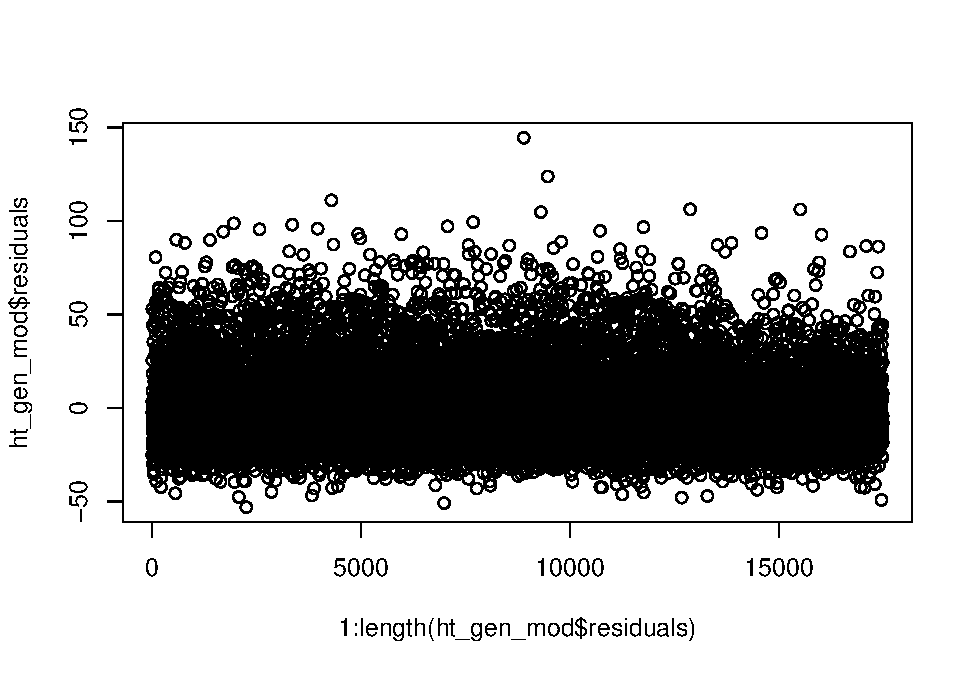
\includegraphics{MA206supplement_files/figure-latex/unnamed-chunk-7-1.pdf}

The following figure depicts the residuals vs fitted values from our model with both height and Sex. The residuals do not show a pattern and are scattered roughly equally above and below the \(y = 0\) line. It seems reasonable to believe that the linearity validity condition is met.

\begin{Shaded}
\begin{Highlighting}[]
\KeywordTok{plot}\NormalTok{(ht_gen_mod}\OperatorTok{$}\NormalTok{fitted,ht_gen_mod}\OperatorTok{$}\NormalTok{residuals)}
\end{Highlighting}
\end{Shaded}

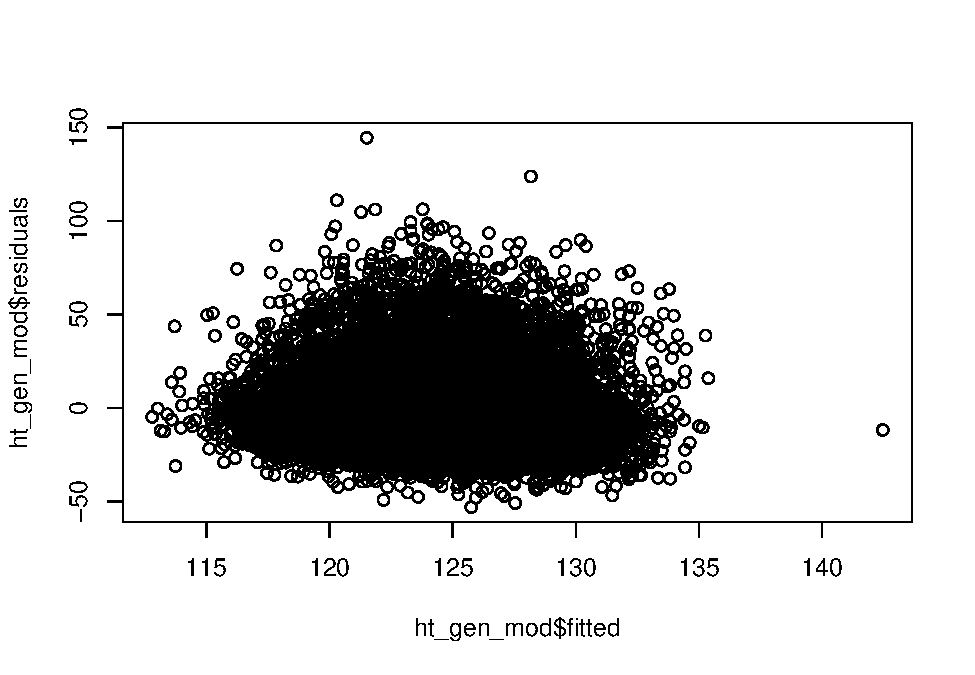
\includegraphics{MA206supplement_files/figure-latex/unnamed-chunk-8-1.pdf}

From this same plot, we see the variance of the residuals is relatively constant as our predicted SBP increases. The validity condition requiring equal variance seems reasonable.

The histogram of our residuals looks relatively normal although it does seem to have a heavy right tail. Our residuals may not be strictly normal. However, linear regression is ``robust'' to departures from normality. That means that slight, or even moderate, departures from normality generally do not pose a problem. Our residuals look ``normal enough'' that I feel comfortable concluding that our validity conditions are met.

\begin{Shaded}
\begin{Highlighting}[]
\KeywordTok{hist}\NormalTok{(ht_gen_mod}\OperatorTok{$}\NormalTok{resid)}
\end{Highlighting}
\end{Shaded}

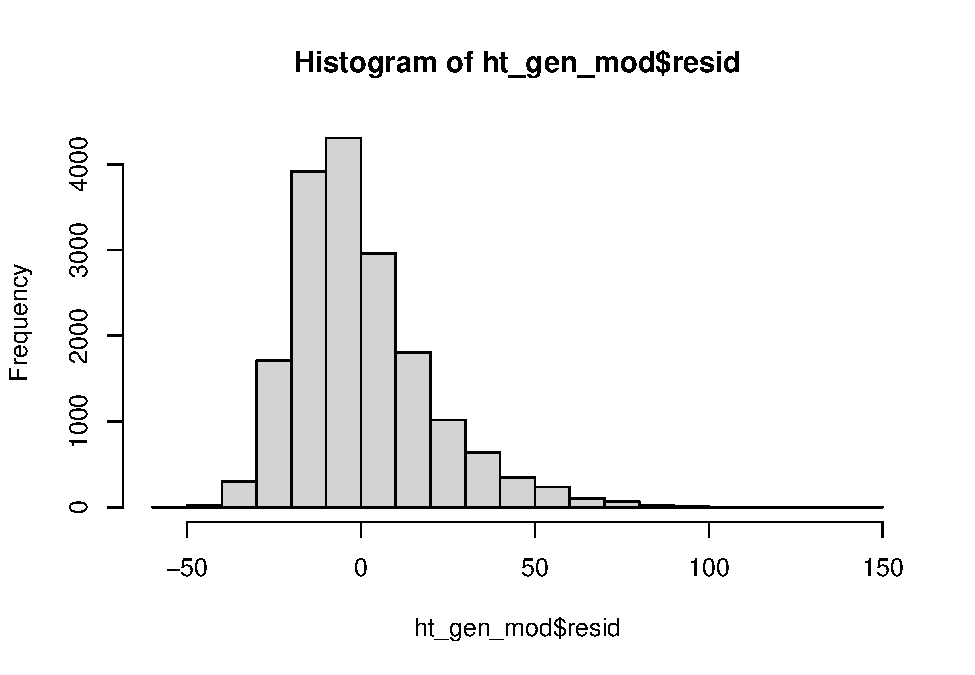
\includegraphics{MA206supplement_files/figure-latex/unnamed-chunk-9-1.pdf}

What would we expect to see if the validity conditions were violated? Below are some examples of model diagnostic plots that indicate a departure from our validity conditions. We simulated the data used to create these plots so we know which conditions are not valid. These are also relatively extreme examples for illustrative purposes; in real data you often will not see patterns this obvious. Violations of our model's validity conditions can be especially hard to detect when we have a small sample size.

First, we look at independence. The following plot of residuals in order show a clear pattern. The residuals seem to be in triplets; first we have a positive residual, then a residual around zero, then a negative residual. This pattern indicates that are model is missing an important factor, like time. Perhaps the data was a reading collected three times a day - morning, noon and night - and we expect the reading will differ based on time of day but we did not include that in the model. Departures from independence are rarely this easy to spot.

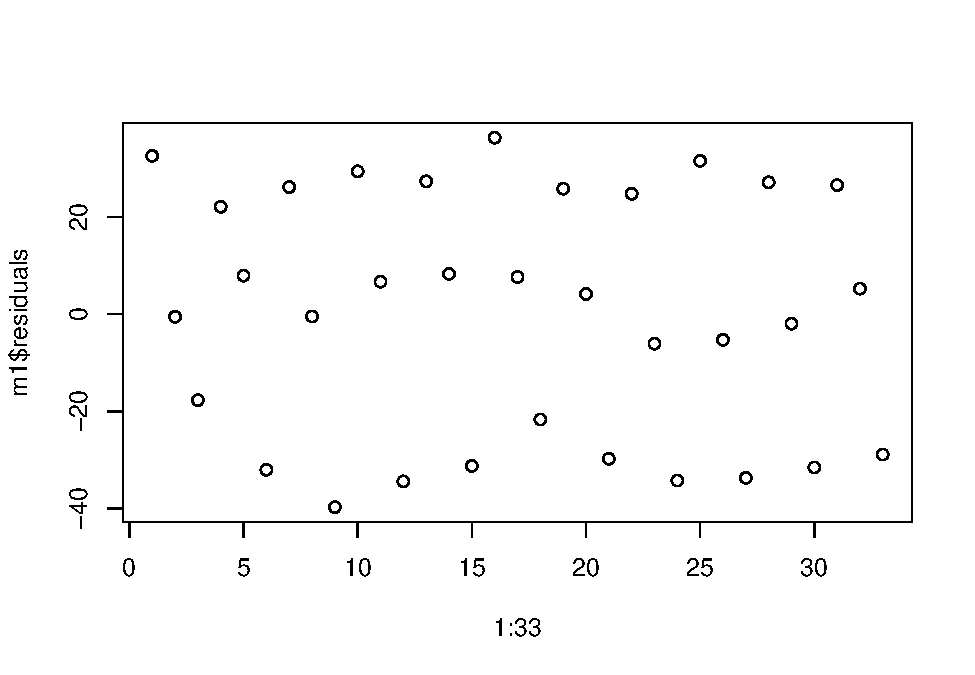
\includegraphics{MA206supplement_files/figure-latex/unnamed-chunk-10-1.pdf}

--\textgreater{}

Next we look at the linearity assumption. Below we see a residuals vs fitted values plot that shows a clear pattern. Fitted values below about 150 or above about 350 tend to have positive residuals (i.e.~be underestimated) whereas fitted values between 150 and 350 tend to have negative residuals (i.e.~be overestimated). This is an indication that our linearity assumption is violated; the right hand side of the model is not correctly specified.

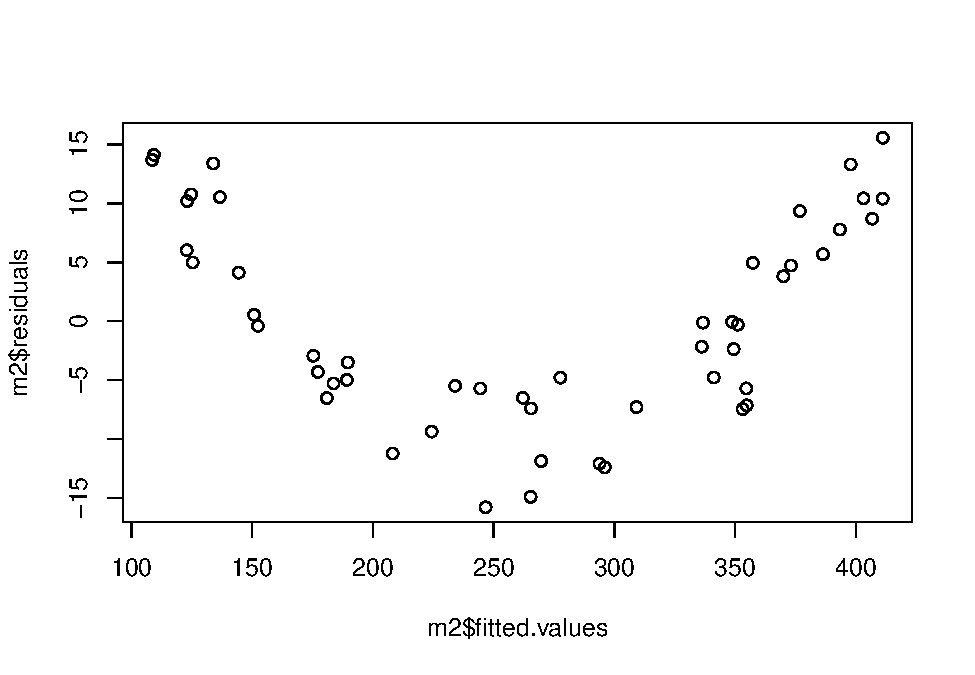
\includegraphics{MA206supplement_files/figure-latex/unnamed-chunk-12-1.pdf}

--\textgreater{}

Next we investigate our assumption of constant variance. In the plot below, we see a clear fanning out of the residuals; as \(\hat{y}\) increases, the variance of the residuals decreases.

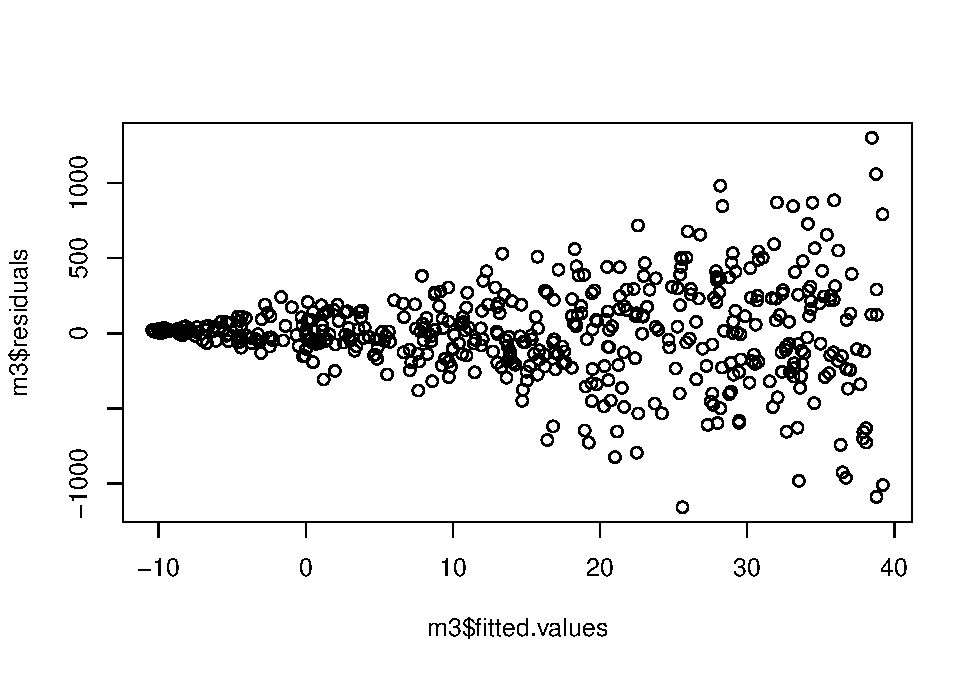
\includegraphics{MA206supplement_files/figure-latex/unnamed-chunk-14-1.pdf}

And finally, we investigate our normality assumption. In the plot below, we see that are residuals are heavily skewed to the right. The assumption of normality is violated.

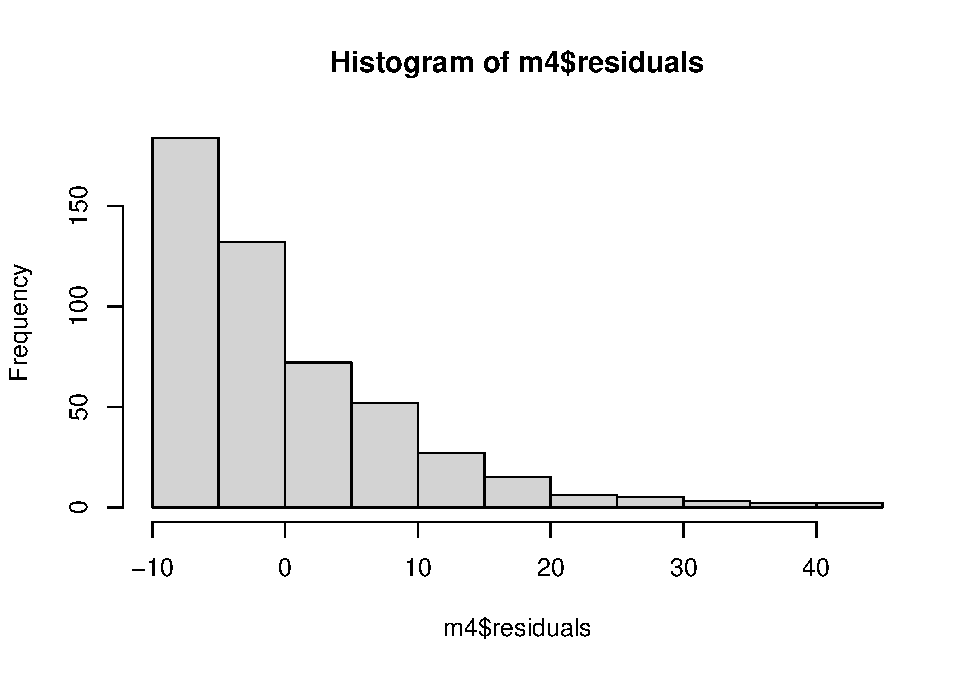
\includegraphics{MA206supplement_files/figure-latex/unnamed-chunk-15-1.pdf}

In our example, researchers were specifically interested in the relationship between height and blood pressure so height was our treatment variable. Sex was related to both height and blood pressure so we need to include it in our model, but we are not particularly interested in the relationship between Sex and blood pressure from a clinical or scientific standpoint. So Sex was a confounding variable. Notice that we treat these variables the same from a statistical standpoint. It is possible to have multiple exposures or treatments, multiple confounders, or both. The distinction between the two is not a statistical one; it is a scientific one.\\

\hypertarget{quantitative-confounding-variable}{%
\section{Quantitative confounding variable}\label{quantitative-confounding-variable}}

Confounding variables can, of course, be quantitative as well. Here we will explore the situation where you have a quantitative treatment variable \((X)\), a quantitative response variable \((Y)\), and a quantitative confounding variable \((C)\). In fact, the ice cream example from the chapter 4 was just such a situation.

\hypertarget{unadjusted-effect-of-x-on-y-1}{%
\subsection{\texorpdfstring{Unadjusted effect of \(X\) on \(Y\)}{Unadjusted effect of X on Y}}\label{unadjusted-effect-of-x-on-y-1}}

The file wage\_data.csv {[}ROB, can you either post this to course website or\ldots{}? Actually, there isn't really an ``or'' I guess.{]} on the course website contains a subset of wage data from the Center for Economic and Policy Research. It includes individual annual income from wages and salary (Earnings) for people who are above the poverty line but below the ``top 2\%''. {[}Do you think I should cite info for pverty line and top 2\%?{]} We wish to explore the relationship between family size and earnings. A scatterplot indicates that there does appear to be a positive relationship between the two variables.

\begin{Shaded}
\begin{Highlighting}[]
\NormalTok{wage_dat<-}\KeywordTok{read_csv}\NormalTok{(}\StringTok{"./data/wage_data.csv"}\NormalTok{)}
\end{Highlighting}
\end{Shaded}

\begin{verbatim}
## Parsed with column specification:
## cols(
##   .default = col_double(),
##   Education = col_character(),
##   Sex = col_character(),
##   MaritalStatus = col_character(),
##   Race = col_character(),
##   FamilyMakeup = col_character()
## )
\end{verbatim}

\begin{verbatim}
## See spec(...) for full column specifications.
\end{verbatim}

\begin{Shaded}
\begin{Highlighting}[]
\NormalTok{wage_dat}\OperatorTok
\StringTok{  }\KeywordTok{ggplot}\NormalTok{(}\KeywordTok{aes}\NormalTok{(}\DataTypeTok{x=}\NormalTok{FamilySize, }\DataTypeTok{y=}\NormalTok{Earnings))}\OperatorTok{+}
\StringTok{  }\KeywordTok{geom_point}\NormalTok{()}\OperatorTok{+}
\StringTok{  }\KeywordTok{labs}\NormalTok{(}\DataTypeTok{x=}\StringTok{"Family Size"}\NormalTok{, }\DataTypeTok{y =} \StringTok{"Annual Earnings"}\NormalTok{, }\DataTypeTok{title =} \StringTok{"Family Size versus Annual Earnings"}\NormalTok{)}
\end{Highlighting}
\end{Shaded}

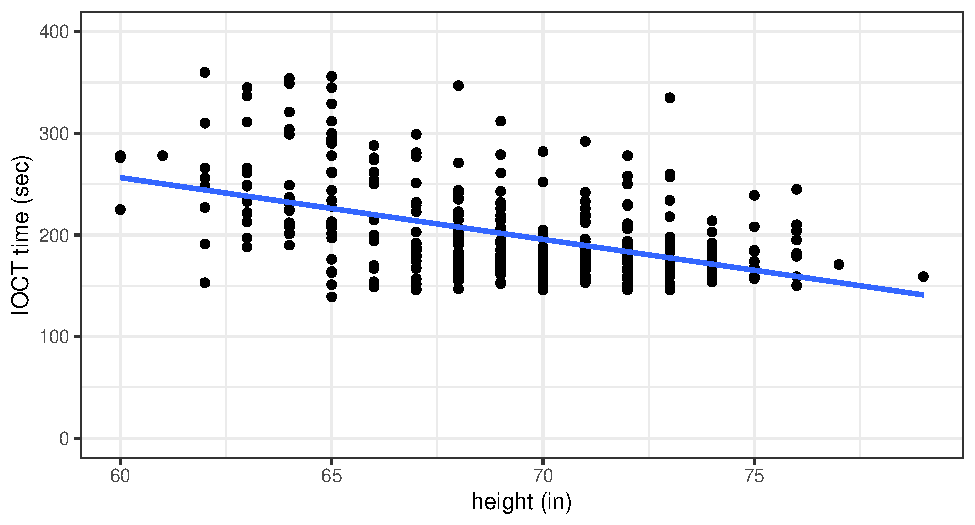
\includegraphics{MA206supplement_files/figure-latex/unnamed-chunk-16-1.pdf}

If we were to consider only the treatment variable FamilySize and the response variable Earnings, we could use the following regression equation:
\[\widehat{Earnings} = \beta_0+\beta_1*FamilySize\]
Fitting this in R, we get the following results:

\begin{Shaded}
\begin{Highlighting}[]
\NormalTok{size_mod =}\StringTok{ }\KeywordTok{lm}\NormalTok{(Earnings}\OperatorTok{~}\NormalTok{FamilySize, }\DataTypeTok{data =}\NormalTok{ wage_dat)}
\KeywordTok{summary}\NormalTok{(size_mod)}
\end{Highlighting}
\end{Shaded}

\begin{verbatim}
## 
## Call:
## lm(formula = Earnings ~ FamilySize, data = wage_dat)
## 
## Residuals:
##    Min     1Q Median     3Q    Max 
## -41825 -28222 -13021  13383 141580 
## 
## Coefficients:
##             Estimate Std. Error t value Pr(>|t|)    
## (Intercept)    49012       4212  11.636  < 2e-16 ***
## FamilySize      4802       1272   3.775 0.000179 ***
## ---
## Signif. codes:  0 '***' 0.001 '**' 0.01 '*' 0.05 '.' 0.1 ' ' 1
## 
## Residual standard error: 39120 on 498 degrees of freedom
## Multiple R-squared:  0.02782,    Adjusted R-squared:  0.02587 
## F-statistic: 14.25 on 1 and 498 DF,  p-value: 0.0001792
\end{verbatim}

We see that there is a very significant effect of family size on earnings; for every additional member of the family, we expect to earn about \$48702 more.

\hypertarget{effect-of-x-on-y-adjusting-for-c-1}{%
\subsection{\texorpdfstring{Effect of \(X\) on \(Y\) adjusting for \(C\)}{Effect of X on Y adjusting for C}}\label{effect-of-x-on-y-adjusting-for-c-1}}

However, there are a number of factors that are related to both earnings and family size, perhaps in a causal way. We will look at age. We expect to earn more as we age and get more experience in the workforce and possibly even more education. We also expect that, in general, family size will increase - or at least stay the same - as we get older. We can visually inspect our data to check this. Below is a graph of earnings versus age.

\begin{Shaded}
\begin{Highlighting}[]
\NormalTok{wage_dat}\OperatorTok
\StringTok{  }\KeywordTok{ggplot}\NormalTok{(}\KeywordTok{aes}\NormalTok{(}\DataTypeTok{x=}\StringTok{`}\DataTypeTok{Age}\StringTok{`}\NormalTok{,}
             \DataTypeTok{y=}\StringTok{`}\DataTypeTok{Earnings}\StringTok{`}\NormalTok{))}\OperatorTok{+}
\StringTok{  }\KeywordTok{geom_point}\NormalTok{()}\OperatorTok{+}
\StringTok{  }\KeywordTok{geom_smooth}\NormalTok{(}\DataTypeTok{method =} \StringTok{"lm"}\NormalTok{, }\DataTypeTok{se=}\OtherTok{FALSE}\NormalTok{)}\OperatorTok{+}
\StringTok{  }\KeywordTok{theme_classic}\NormalTok{()}
\end{Highlighting}
\end{Shaded}

\begin{verbatim}
## `geom_smooth()` using formula 'y ~ x'
\end{verbatim}

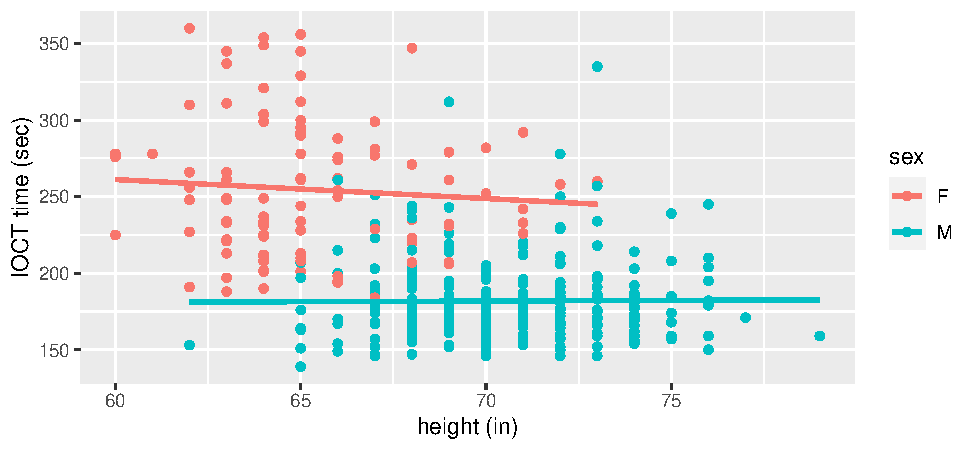
\includegraphics{MA206supplement_files/figure-latex/unnamed-chunk-18-1.pdf}

Age is a potential \emph{confounder}. When we add age to the model with family size, we have the following regression model:

\[\widehat{Earnings}=\beta_0+\beta_1*FamilySize+\beta_2*Age\]
When we estimate the coefficents for this model in R, we get the following results.

\begin{Shaded}
\begin{Highlighting}[]
\NormalTok{size_age_mod =}\StringTok{ }\KeywordTok{lm}\NormalTok{(Earnings}\OperatorTok{~}\NormalTok{FamilySize}\OperatorTok{+}\NormalTok{Age, }\DataTypeTok{data =}\NormalTok{ wage_dat)}
\KeywordTok{summary}\NormalTok{(size_age_mod)}
\end{Highlighting}
\end{Shaded}

\begin{verbatim}
## 
## Call:
## lm(formula = Earnings ~ FamilySize + Age, data = wage_dat)
## 
## Residuals:
##    Min     1Q Median     3Q    Max 
## -48975 -26711 -12103  14107 145564 
## 
## Coefficients:
##             Estimate Std. Error t value Pr(>|t|)    
## (Intercept)  26643.8     8322.0   3.202  0.00145 ** 
## FamilySize    5534.1     1283.0   4.314 1.94e-05 ***
## Age            449.7      144.7   3.107  0.00199 ** 
## ---
## Signif. codes:  0 '***' 0.001 '**' 0.01 '*' 0.05 '.' 0.1 ' ' 1
## 
## Residual standard error: 38790 on 497 degrees of freedom
## Multiple R-squared:  0.04635,    Adjusted R-squared:  0.04251 
## F-statistic: 12.08 on 2 and 497 DF,  p-value: 7.551e-06
\end{verbatim}

We see that there is still a significant positive effect of family size on earnings, although it's magnitude is slightly larger. We expect to earn about \$5534 less per year for every additional member of the family \emph{after adjusting for age}. We also note that the coefficient for age is 449.7, meaning that, for every year older a person is, we expect them to earn \$450 more on average, after adjusting for family size. Of course, the relationship between family size and earnings is a complex one that would require a much more extensive analysis to fully understand.

\hypertarget{assessing-model-adequacy-1}{%
\subsection{Assessing model adequacy}\label{assessing-model-adequacy-1}}

Just like with previous regression models, these results might not mean much if our validity conditions aren't met.

Here, we may be willing to believe that our assumption of independence is met by the way the data was collected. The CEPR data is from the CPS, a monthly survey\ldots{}.{[}ROB - put stuff here please!{]} and this subset is a random sample of the overall CPS from {[}ROB!{]}

To check for linearity and equal variance, we can plot the predicted values vs.~the residuals.

\begin{Shaded}
\begin{Highlighting}[]
\NormalTok{size_age_mod}\OperatorTok
\StringTok{  }\KeywordTok{fortify}\NormalTok{(wage_dat)}\OperatorTok
\StringTok{  }\KeywordTok{ggplot}\NormalTok{(}\KeywordTok{aes}\NormalTok{(}\DataTypeTok{x =}\NormalTok{ .fitted, }\DataTypeTok{y =}\NormalTok{ .resid))}\OperatorTok{+}
\StringTok{  }\KeywordTok{geom_point}\NormalTok{()}\OperatorTok{+}
\StringTok{  }\KeywordTok{geom_hline}\NormalTok{(}\DataTypeTok{yintercept =} \DecValTok{0}\NormalTok{)}\OperatorTok{+}
\StringTok{  }\KeywordTok{labs}\NormalTok{( }\DataTypeTok{x =} \StringTok{"Predicted Values"}\NormalTok{, }\DataTypeTok{y =} \StringTok{"Residuals"}\NormalTok{, }\DataTypeTok{title =} \StringTok{"Residuals vs. predicted values"}\NormalTok{)}
\end{Highlighting}
\end{Shaded}

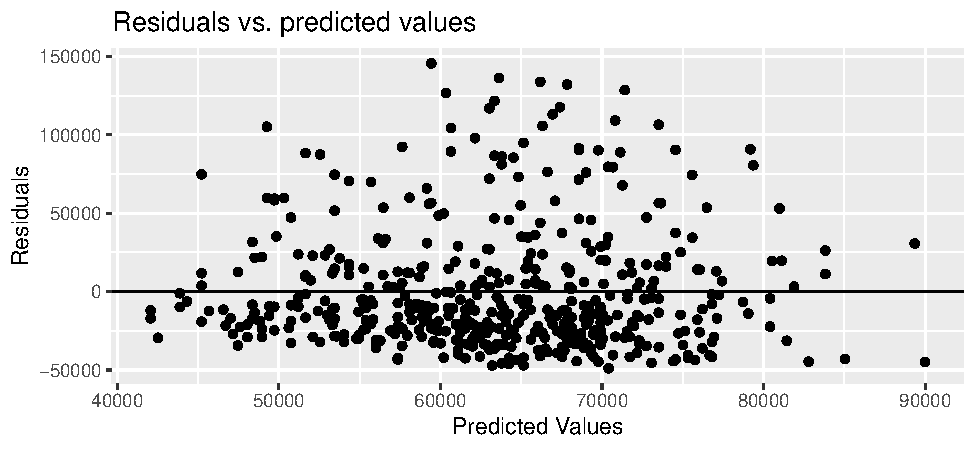
\includegraphics{MA206supplement_files/figure-latex/unnamed-chunk-20-1.pdf}

The linearity and constant variance conditions appear to be met. Although we have some large positive residuals, there does not appear to be a pattern and the width is relatively constant.

Our histogram, however, shows that the residuals seem to be skewed relatively heavily to the right. Our fourth validity condition, normality of the residuals, is likely not met. Although we can be comfortable in our estimates of the regression coefficients, we should be careful about drawing any conclusions about their statistical significance. (For a much more in depth assumption about assessing model adequacy, to include methods to handle violations of the validity conditions, take MA376!)

\begin{Shaded}
\begin{Highlighting}[]
\KeywordTok{hist}\NormalTok{(size_age_mod}\OperatorTok{$}\NormalTok{residuals)}
\end{Highlighting}
\end{Shaded}

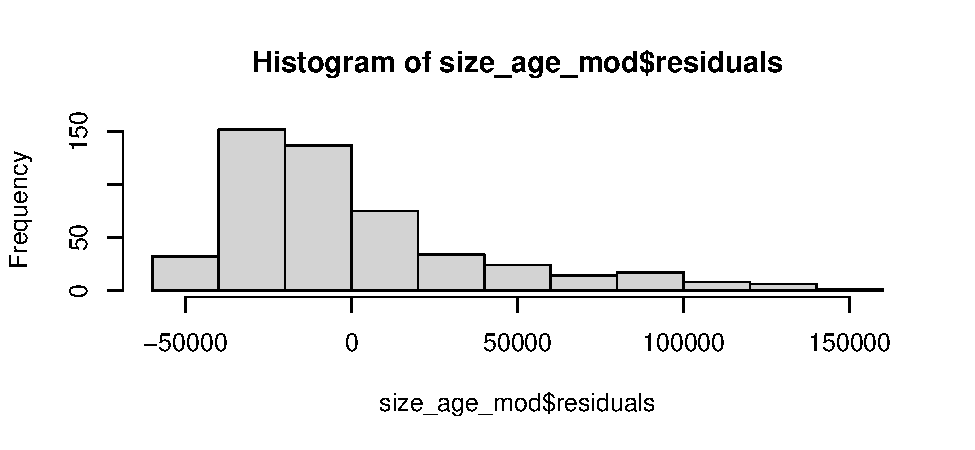
\includegraphics{MA206supplement_files/figure-latex/unnamed-chunk-21-1.pdf}

\hypertarget{activity}{%
\chapter{Activity}\label{activity}}

\emph{Title}: The Indoor Obstacle Course Test (IOCT)

\emph{Topics}\}*: Confounding, Causal Diagrams, Simple Linear Regression, Confidence Intervals

\emph{Background}: Cadets at West Point must pass the \href{https://www.youtube.com/watch?v=94tPO0fGtJo\&t=77s}{Indoor Obstacle Course Test} (IOCT) to graduate. The IOCT begins with a series of floor and climbing obstacles and ends with several laps around an indoor track. It is an exhausting test of endurance and strength. In addition to being a graduation requirement, cadets receive a letter grade that is factored into their class rank.

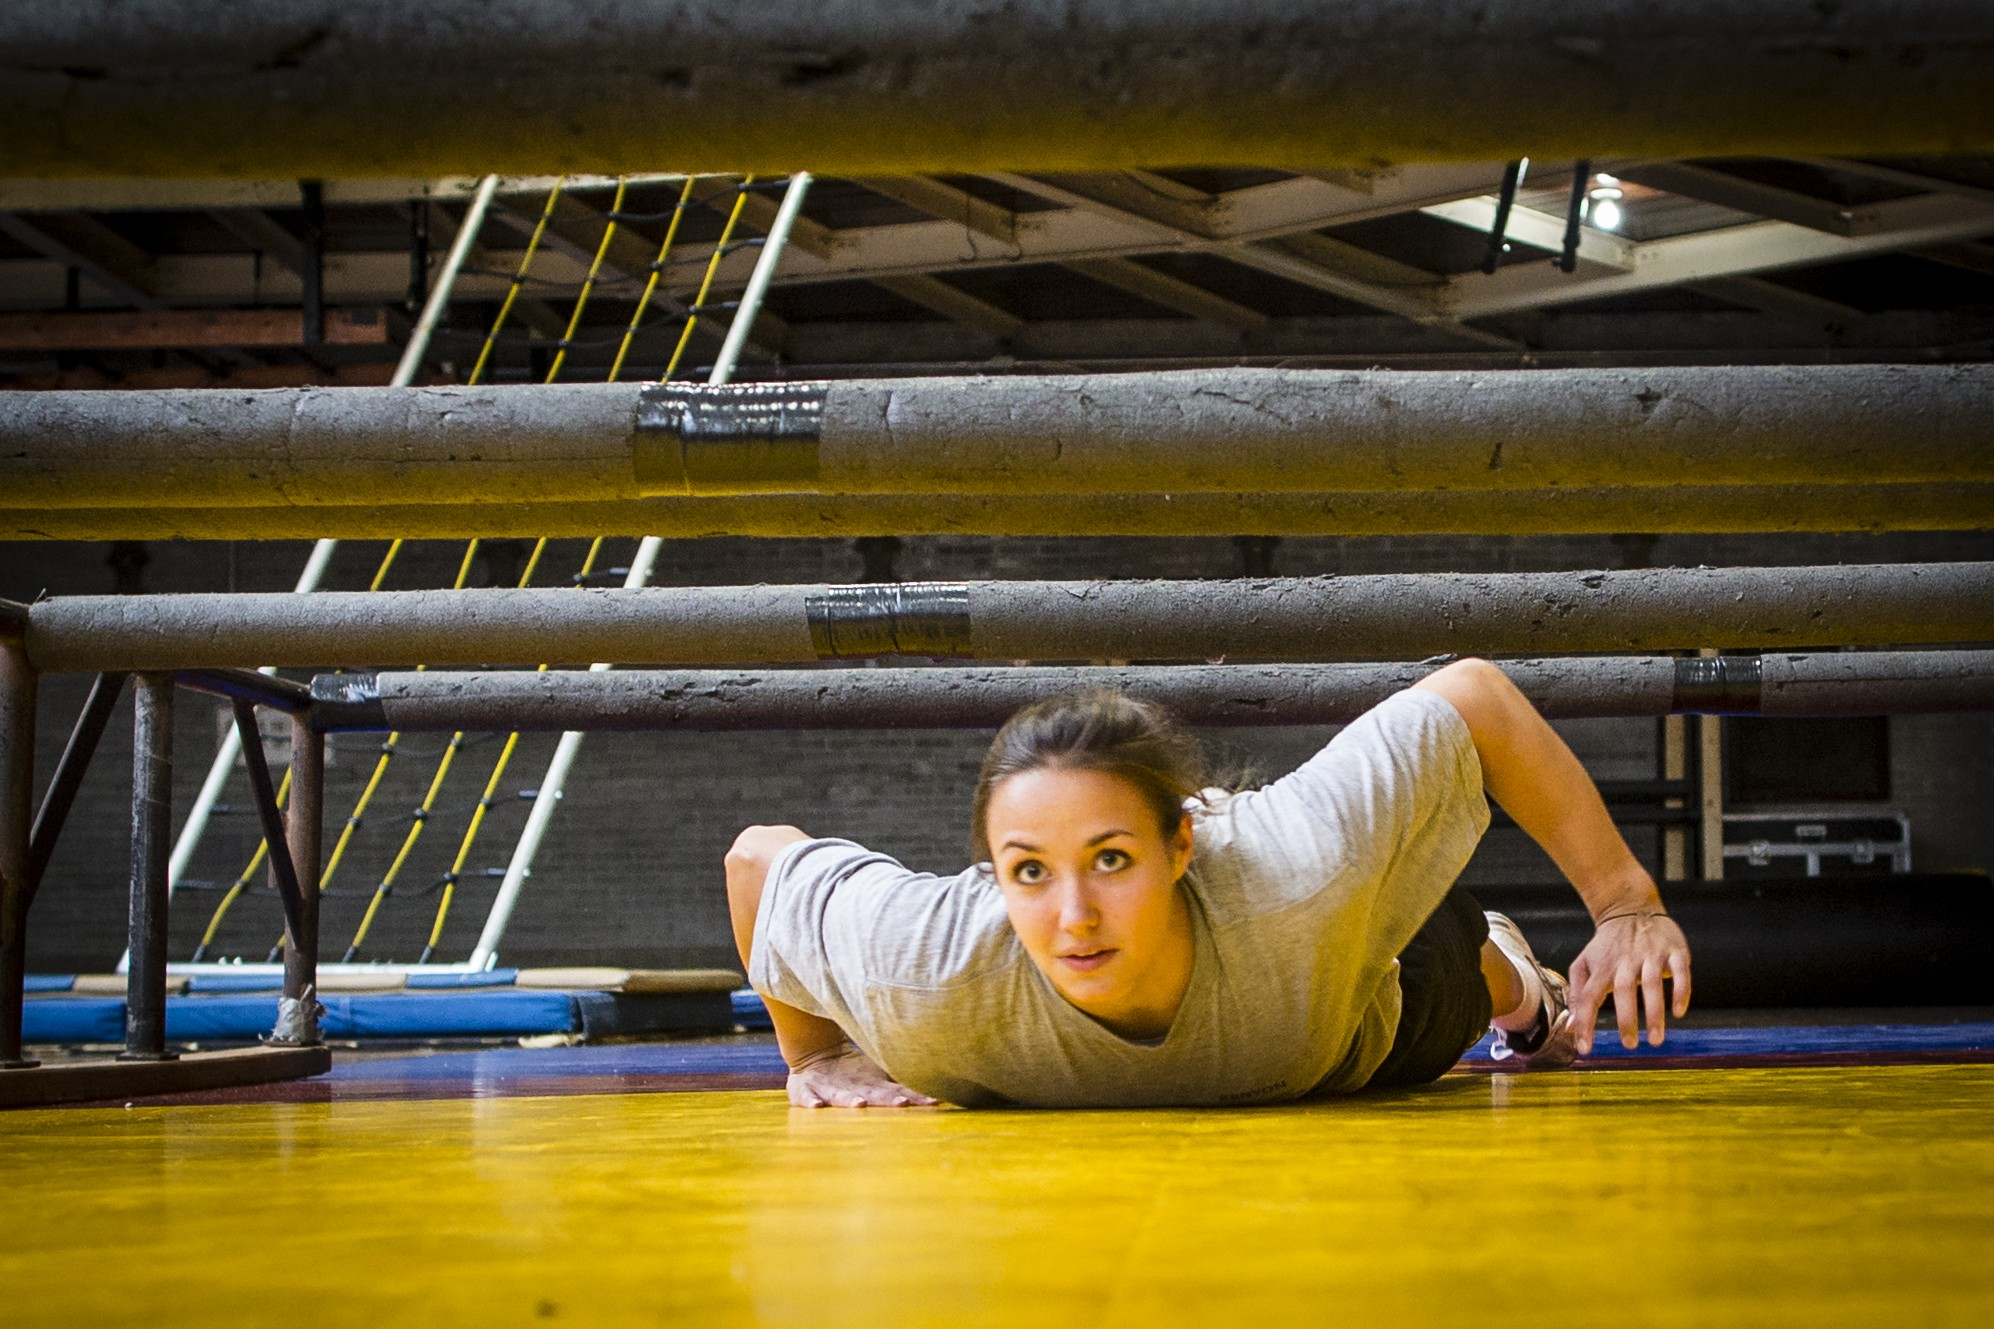
\includegraphics[width=0.5\textwidth,height=\textheight]{./images/crawlObstacle.jpg} 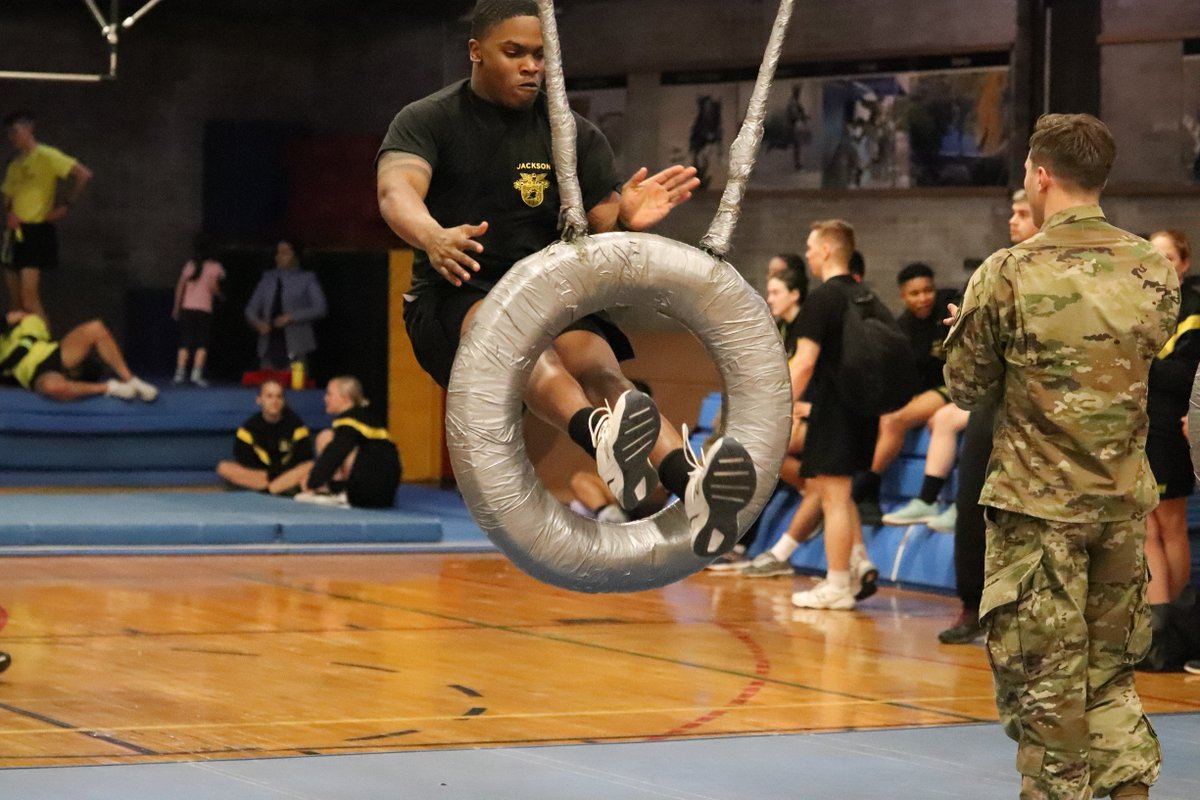
\includegraphics[width=0.5\textwidth,height=\textheight]{./images/tireObstacle.jpg}

Shorter cadets often argue they are at a disadvantage on the obstacle course. Many obstacles appear to favor taller cadets because they are easier to reach. In this study, we will investigate the effect of height on IOCT times.

\begin{enumerate}
\def\labelenumi{\arabic{enumi}.}
\tightlist
\item
  \href{https://www.youtube.com/watch?v=94tPO0fGtJo\&t=77s}{Watch the video of Cadet Madaline Kenyon running the IOCT}. In your opinion, do some obstacles favor taller cadets? Explain.
\end{enumerate}

\vspace{1in}

The file \texttt{obstacle\_course.csv} contains height (inches), IOCT times (seconds), biological sex (M/F), and whether the cadet played an intercollegiate sport for a sample of 384 cadets who ran the IOCT course in the last five years.

\begin{enumerate}
\def\labelenumi{\arabic{enumi}.}
\setcounter{enumi}{1}
\tightlist
\item
  What is the explanatory variable in this study? Classify the variable as quantitative or categorical.
\end{enumerate}

\vspace{0.25in}

\begin{enumerate}
\def\labelenumi{\arabic{enumi}.}
\setcounter{enumi}{2}
\tightlist
\item
  What is the response variable in this study? Classify the variable as quantitative or categorical.
\end{enumerate}

\vspace{0.25in}

\begin{enumerate}
\def\labelenumi{\arabic{enumi}.}
\setcounter{enumi}{3}
\tightlist
\item
  Is this study an observational study or a randomized experiment? Explain.
\end{enumerate}

\vspace{1in}

\newpage

Figure 1 depicts IOCT times in seconds versus height in inches. Table 1 contains information from the linear regression model.

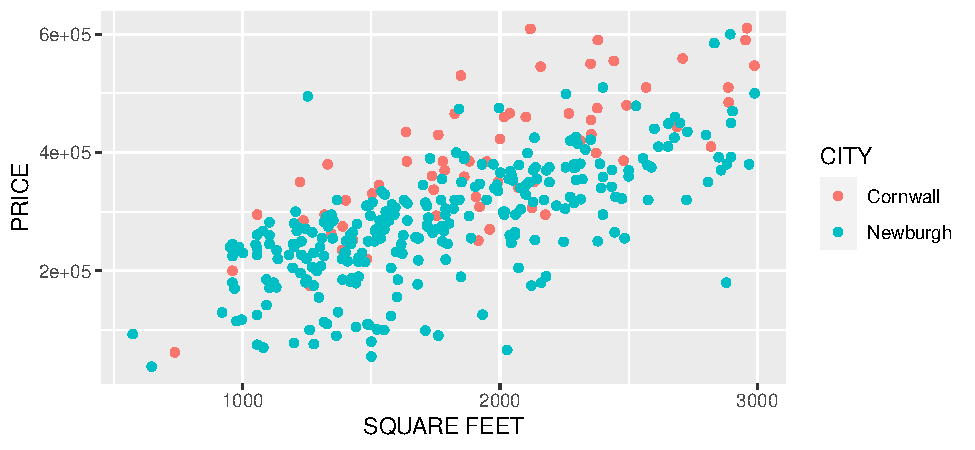
\includegraphics{MA206supplement_files/figure-latex/unnamed-chunk-22-1.pdf}

\begin{table}

\caption{\label{tab:unnamed-chunk-22}Linear regression output for IOCT times and height.}
\centering
\begin{tabular}[t]{l|r|r|r|r}
\hline
term & estimate & std.error & statistic & p.value\\
\hline
(Intercept) & 621.00 & 39.98 & 15.53 & 0\\
\hline
height & -6.08 & 0.58 & -10.52 & 0\\
\hline
\end{tabular}
\end{table}

\begin{enumerate}
\def\labelenumi{\arabic{enumi}.}
\setcounter{enumi}{4}
\item
  Interpret the estimate of the height coefficient in Table 1.

  \vspace{1in}
\item
  Calculate and interpret a 95\% confidence interval for the slope coefficient.
\end{enumerate}

\vspace{1in}

\newpage

\begin{enumerate}
\def\labelenumi{\arabic{enumi}.}
\setcounter{enumi}{6}
\tightlist
\item
  The \(p\)-value for height in Table 1 indicates there is strong evidence of an association between height and IOCT time. Taller cadets tend to do better on the IOCT. Some people would say the result is \emph{statistically significant}. However, statistical significance and practical signifigance are different. \href{https://en.wikipedia.org/wiki/Indoor_Obstacle_Course_Test}{Review the grade scale for the IOCT.} In your opinion, does the observed association have practical significance? Explain.
\end{enumerate}

\vspace{1in}

\begin{enumerate}
\def\labelenumi{\arabic{enumi}.}
\setcounter{enumi}{7}
\tightlist
\item
  A shorter cadet argues Figure 1 shows evidence the IOCT is unfair based on height. Do you agree or disagree? Explain.
\end{enumerate}

\vspace{1in}

\begin{enumerate}
\def\labelenumi{\arabic{enumi}.}
\setcounter{enumi}{8}
\tightlist
\item
  Briefly explain the difference between these two conclusions.
\end{enumerate}

\begin{itemize}
\item
  \emph{Height is associated with faster IOCT times.}
\item
  \emph{Height causes faster IOCT times.}
\end{itemize}

\vspace{1in}

\begin{enumerate}
\def\labelenumi{\arabic{enumi}.}
\setcounter{enumi}{9}
\tightlist
\item
  Based on the analysis presented thus far, is it possible to distinguish between these two explanations? Explain.
\end{enumerate}

\vspace{1in}

\begin{enumerate}
\def\labelenumi{\arabic{enumi}.}
\setcounter{enumi}{10}
\tightlist
\item
  Draw a causal diagram depicting the relationship between height, IOCT time, and sex. Explain your decisions to include/exclude arrows in the diagram.
\end{enumerate}

\vspace{1in}

\begin{enumerate}
\def\labelenumi{\arabic{enumi}.}
\setcounter{enumi}{11}
\tightlist
\item
  Based on your diagram, identify the confounding variable.
\end{enumerate}

\vspace{0.5in}

Below are boxplots of height in inches and IOCT times in seconds by sex.

\begin{figure}
\centering
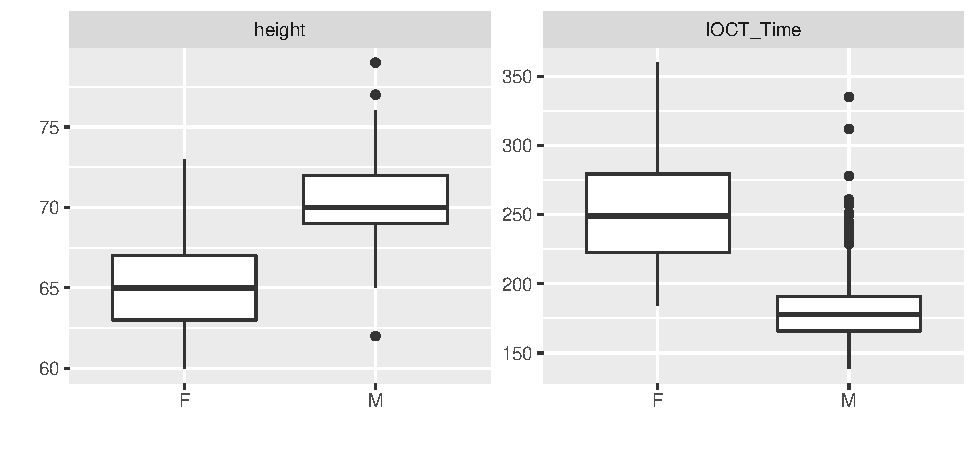
\includegraphics{MA206supplement_files/figure-latex/unnamed-chunk-23-1.pdf}
\caption{\label{fig:unnamed-chunk-23}Height (inches) and IOCT time (seconds) by sex.}
\end{figure}

\begin{enumerate}
\def\labelenumi{\arabic{enumi}.}
\setcounter{enumi}{12}
\tightlist
\item
  Based on Figure 2, is the estimate of the effect of height on IOCT time in Table 1 confounded by sex? If so, is the effect of height smaller or larger than that reported in Table 1? Explain.
\end{enumerate}

\vspace{1in}

\newpage

Figure 3 depicts the association between IOCT time and height by sex. Tables 2 and 3 depict regression results for female and male cadets, respectively.

\begin{figure}
\centering
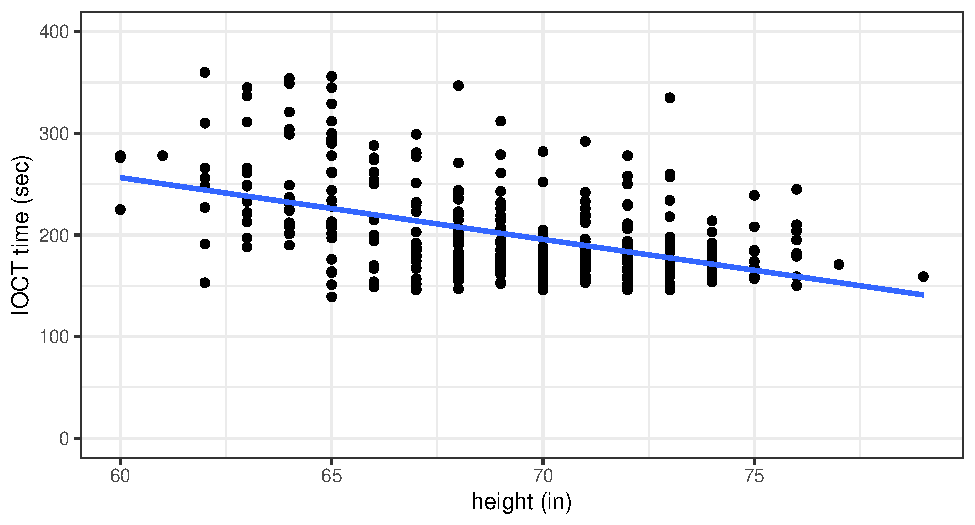
\includegraphics{MA206supplement_files/figure-latex/unnamed-chunk-24-1.pdf}
\caption{\label{fig:unnamed-chunk-24}Indoor Obstacle Course Test (IOCT) times versus height by sex (n = 384).}
\end{figure}

\begin{table}

\caption{\label{tab:unnamed-chunk-25}Regression results for female cadets.}
\centering
\begin{tabular}[t]{l|r|r|r|r}
\hline
term & estimate & std.error & statistic & p.value\\
\hline
(Intercept) & 335.76 & 107.44 & 3.12 & 0.00\\
\hline
height & -1.24 & 1.64 & -0.76 & 0.45\\
\hline
\end{tabular}
\end{table}

\begin{table}

\caption{\label{tab:unnamed-chunk-25}Regression results for male cadets.}
\centering
\begin{tabular}[t]{l|r|r|r|r}
\hline
term & estimate & std.error & statistic & p.value\\
\hline
(Intercept) & 175.61 & 40.92 & 4.29 & 0.00\\
\hline
height & 0.09 & 0.58 & 0.15 & 0.88\\
\hline
\end{tabular}
\end{table}

\begin{enumerate}
\def\labelenumi{\arabic{enumi}.}
\setcounter{enumi}{13}
\tightlist
\item
  Based on Figure 3 and Tables 2 and 3, does it appear there is an association between IOCT time and height within levels of sex? Explain.
\end{enumerate}

\vspace{1in}

\newpage

\begin{enumerate}
\def\labelenumi{\arabic{enumi}.}
\setcounter{enumi}{14}
\tightlist
\item
  In your opinion, is there much evidence that height is an advantage on the IOCT (in other words, is height the \emph{cause} of better IOCT times)? Explain.
\end{enumerate}

\vspace{2in}

\begin{enumerate}
\def\labelenumi{\arabic{enumi}.}
\setcounter{enumi}{15}
\tightlist
\item
  Briefly discuss two ways you could improve this study to better assess whether there is a height advantage.
\end{enumerate}

\vspace{1in}

\bibliography{book.bib,packages.bib}

\end{document}
